% ============================================================================
% QUANTUM FOOD OPTIMIZATION - 5-MINUTE PRESENTATION
% Condensed Version for OQI Showcase
% Author: Edoardo Spigarolo
% ============================================================================

\documentclass[aspectratio=169,10pt]{beamer}

% ============================================================================
% THEME AND COLORS
% ============================================================================
\usetheme{default}
\usecolortheme{default}

% Custom colors - Professional blue-green quantum theme
\definecolor{primaryBlue}{RGB}{0, 84, 147}
\definecolor{secondaryBlue}{RGB}{0, 119, 182}
\definecolor{accentTeal}{RGB}{0, 150, 136}
\definecolor{accentGreen}{RGB}{76, 175, 80}
\definecolor{warmOrange}{RGB}{255, 152, 0}
\definecolor{alertRed}{RGB}{244, 67, 54}
\definecolor{lightBg}{RGB}{245, 248, 250}
\definecolor{darkText}{RGB}{33, 37, 41}
\definecolor{mutedGray}{RGB}{108, 117, 125}

% Set main colors
\setbeamercolor{palette primary}{bg=primaryBlue,fg=white}
\setbeamercolor{palette secondary}{bg=secondaryBlue,fg=white}
\setbeamercolor{palette tertiary}{bg=accentTeal,fg=white}
\setbeamercolor{structure}{fg=primaryBlue}
\setbeamercolor{title}{fg=white}
\setbeamercolor{frametitle}{fg=primaryBlue,bg=white}
\setbeamercolor{normal text}{fg=darkText}
\setbeamercolor{block title}{bg=primaryBlue,fg=white}
\setbeamercolor{block body}{bg=lightBg,fg=darkText}
\setbeamercolor{block title example}{bg=accentGreen,fg=white}
\setbeamercolor{block body example}{bg=lightBg,fg=darkText}
\setbeamercolor{block title alerted}{bg=alertRed,fg=white}
\setbeamercolor{block body alerted}{bg=lightBg,fg=darkText}
\setbeamercolor{itemize item}{fg=primaryBlue}
\setbeamercolor{itemize subitem}{fg=secondaryBlue}
\setbeamercolor{enumerate item}{fg=primaryBlue}

% ============================================================================
% PACKAGES
% ============================================================================
\usepackage[utf8]{inputenc}
\usepackage[T1]{fontenc}
\usepackage{lmodern}
\usepackage{amsmath,amssymb,amsfonts}
\usepackage{graphicx}
\usepackage{tikz}
\usetikzlibrary{shapes,arrows,positioning,calc,decorations.pathmorphing,backgrounds,fit,automata,shadows,patterns,arrows.meta}
\usepackage{pgfplots}
\pgfplotsset{compat=1.18}
\usepackage{booktabs}
\usepackage{multirow}
\usepackage{array}
\usepackage{xcolor}
\usepackage{fontawesome5}
\usepackage{tcolorbox}
\tcbuselibrary{skins,breakable}
\usepackage{hyperref}
\usepackage{colortbl}

% Graphics path - use actual location of plots
\graphicspath{{../plots/}{images/}}

% ============================================================================
% CUSTOM BEAMER TEMPLATE
% ============================================================================

% Remove navigation symbols
\setbeamertemplate{navigation symbols}{}

% Reduce margins for denser slides
\setbeamersize{text margin left=0.6cm,text margin right=0.6cm}

% Custom headline with OQI branding
\setbeamertemplate{headline}{%
    \begin{tikzpicture}[remember picture,overlay]
        \fill[white] (current page.north west) rectangle ([yshift=-0.8cm]current page.north east);
        \draw[primaryBlue,line width=0.5pt] ([yshift=-0.8cm]current page.north west) -- ([yshift=-0.8cm]current page.north east);
        % OQI logo on left
\node[anchor=north west] at ([xshift=0.3cm,yshift=-0.0cm]current page.north west) {%
    \includegraphics[height=0.65cm]{oqi_logo.png}%
};

% Logo slot 1 (next to OQI logo)
\node[anchor=north west] at ([xshift=2.1cm,yshift=-0.2cm]current page.north west) {%
    \includegraphics[height=0.3cm]{Logo_EPFL_2019.svg.png}%
};
% Logo slot 2
\node[anchor=north west] at ([xshift=3.4cm,yshift=0.15cm]current page.north west) {%
    \includegraphics[height=1cm]{Logo-GAIN.png}%
};
% Logo slot 3
\node[anchor=north west] at ([xshift=4.7cm,yshift=-0.1cm]current page.north west) {%
    \includegraphics[height=0.48cm]{NITheCS logo.png}%
};
% Logo slot 4 (SVG logo)
\node[anchor=north west] at ([xshift=5.9cm,yshift=-0.05cm]current page.north west) {%
    \includegraphics[height=0.5cm]{qb_logo_rgb_black_nosub.png}%
};
% OQI text on right
\node[anchor=north east] at ([xshift=-0.3cm,yshift=-0.1cm]current page.north east) {%
    \includegraphics[height=0.5cm]{oqi_text.png}%
};
    \end{tikzpicture}
    \vspace{0.8cm}
}

% Custom footline with OQI footer image
\setbeamertemplate{footline}{%
    \begin{tikzpicture}[remember picture,overlay]
        % Footer image spanning full width
        \node[anchor=south,inner sep=0pt] at (current page.south) {%
            \includegraphics[width=1.1\paperwidth,height=0.5cm]{footer.jpg}%
        };
        % Page number overlay
        \node[anchor=south east,text=white,font=\tiny\bfseries] at ([xshift=-0.3cm,yshift=0.1cm]current page.south east) {\insertframenumber/\inserttotalframenumber};
    \end{tikzpicture}
    \vspace{0.6cm}
}

\setbeamertemplate{frametitle}{%
    \begin{beamercolorbox}[wd=\paperwidth,ht=1cm,dp=0.2cm]{frametitle}
        % Conditional vertical alignment
        \ifx\insertframesubtitle\empty
            \vspace{0.4cm} % no subtitle → push title down
        \else
            \vspace{-0.15cm} % subtitle present → pull content up
        \fi
        \hspace{0.2cm}\usebeamerfont{frametitle}\insertframetitle
        \ifx\insertframesubtitle\empty\else
            \par\hspace{0.4cm}{\footnotesize\color{mutedGray}\insertframesubtitle}
        \fi
    \end{beamercolorbox}
}



% Custom itemize bullets
\setbeamertemplate{itemize item}{\footnotesize\raisebox{0.1em}{\tikz\fill[primaryBlue] (0,0) circle (0.12em);}}
\setbeamertemplate{itemize subitem}{\footnotesize\raisebox{0.1em}{\tikz\fill[secondaryBlue] (0,0) circle (0.08em);}}
\setbeamertemplate{itemize subsubitem}{\footnotesize\raisebox{0.1em}{\tikz\draw[accentTeal,thick] (0,0) circle (0.08em);}}


%===========================================================================
% CUSTOM BOXES
% ============================================================================
\newtcolorbox{keybox}[1][]{
    enhanced,colback=accentTeal!8,colframe=accentTeal,
    boxrule=1pt,arc=3pt,left=5pt,right=5pt,top=4pt,bottom=4pt,#1
}
\newtcolorbox{resultbox}[1][]{
    enhanced,colback=accentGreen!8,colframe=accentGreen,
    boxrule=1pt,arc=3pt,left=5pt,right=5pt,top=4pt,bottom=4pt,#1
}
\newtcolorbox{warnbox}[1][]{
    enhanced,colback=warmOrange!8,colframe=warmOrange,
    boxrule=1pt,arc=3pt,left=5pt,right=5pt,top=4pt,bottom=4pt,#1
}


% ============================================================================
% CUSTOM COMMANDS AND ENVIRONMENTS
% ============================================================================

% Highlight box
\newtcolorbox{highlightbox}[1][]{
    enhanced,
    colback=lightBg,
    colframe=primaryBlue,
    boxrule=1.5pt,
    arc=4pt,
    left=6pt,right=6pt,top=5pt,bottom=5pt,
    shadow={1mm}{-1mm}{0mm}{black!20},
    #1
}

% Key insight box
\newtcolorbox{keyinsight}[1][Key Insight]{
    enhanced,
    colback=accentTeal!10,
    colframe=accentTeal,
    boxrule=1.5pt,
    arc=5pt,
    fonttitle=\bfseries\footnotesize\color{white},
    title=#1,
    coltitle=white,
    attach boxed title to top left={xshift=8pt,yshift=-\tcboxedtitleheight/2},
    boxed title style={colback=accentTeal,arc=3pt,boxrule=0pt}
}

% Warning box
\newtcolorbox{warningbox}[1][Warning]{
    enhanced,
    colback=warmOrange!10,
    colframe=warmOrange,
    boxrule=1.5pt,
    arc=5pt,
    fonttitle=\bfseries\footnotesize\color{white},
    title=#1,
    coltitle=white,
    attach boxed title to top left={xshift=8pt,yshift=-\tcboxedtitleheight/2},
    boxed title style={colback=warmOrange,arc=3pt,boxrule=0pt}
}

% Metric display
\newcommand{\metricbox}[3]{%
    \begin{tikzpicture}
        \node[rounded corners=5pt, fill=#3!15, draw=#3, line width=1.5pt, 
              minimum width=2.5cm, minimum height=1.3cm, align=center,
              drop shadow={shadow xshift=0.5mm, shadow yshift=-0.5mm, opacity=0.3}] {
            {\Large\bfseries\color{#3}#1}\\[1pt]
            {\scriptsize\color{darkText}#2}
        };
    \end{tikzpicture}
}

% ============================================================================
% TITLE PAGE SETUP
% ============================================================================
\title[Food Optimization]{\textbf{Food Production Optimization}}
\subtitle{Quantum Annealing for Sustainable Agriculture}
\author{Edoardo Spigarolo and Dean Brand}
\institute{EPFL | Open Quantum Initiative}
\date{January 2026}

% ============================================================================
% DOCUMENT START
% ============================================================================
\begin{document}


{
\setbeamertemplate{headline}{}
\setbeamertemplate{footline}{}
\begin{frame}[plain]
\begin{tikzpicture}[remember picture,overlay]
    % Background gradient
    \node[inner sep=0,anchor=center] at (current page.center)
    {\includegraphics[width=\paperwidth,height=\paperheight]{images/OQI background.jpeg}};

  % Optional: semi-transparent overlay to improve text contrast
  \fill[black,opacity=0.35] (current page.south west) rectangle (current page.north east);
    
    % Main title
    \node[white,font=\fontsize{32}{36}\selectfont\bfseries,align=center] 
        at ([yshift=1.8cm]current page.center) {Food Production Optimization};
    
    % Subtitle
    \node[white!90,font=\large,align=center] 
        at ([yshift=0.5cm]current page.center) {Quantum Computing for Sustainable Agriculture};
    
    % Phase indicator
    % \node[rounded corners=8pt,fill=accentTeal,text=white,font=\small\bfseries,
    %       inner sep=6pt,drop shadow={opacity=0.3}] 
    %     at ([yshift=-0.6cm]current page.center) {Phase 3 \& 4 Report};
    
    % Author
    \node[white,font=\normalsize] at ([yshift=-2cm]current page.center) {Edoardo Spigarolo};
    
    % Institution
    \node[white!70,font=\small] at ([yshift=-2.6cm]current page.center) 
        {$\bullet$\quad Open Quantum Institute \quad$\bullet$\quad January 2026};
    
    % Bottom decoration
    \fill[white,opacity=0.05] (current page.south west) rectangle ([yshift=0.8cm]current page.south east);
    
    % SDG icons at bottom
    \node[white!60,font=\tiny] at ([yshift=0.4cm]current page.south) 
        {\faLeaf\quad SDG 2 \quad$\bullet$\quad SDG 3 \quad$\bullet$\quad SDG 12 \quad$\bullet$\quad SDG 13 \quad\faGlobe};
\end{tikzpicture}
\end{frame}
}

\begin{frame}{The Team \& Partners}
    
    \vspace{-0.1cm}
    \begin{columns}[T]
        
        \begin{column}{0.58\textwidth}
            \small\textbf{Project Team:}
            \begin{itemize}
                \item Edoardo Spigarolo, Vincenzo Savona (EPFL)
                \item Dean Brand, Francesco Petruccione (NITheCS)
                \item Oliver Camp, Sowrya Kilaru (GAIN)
            \end{itemize}
            
            
            \small\textbf{Mission:}
            \begin{itemize}
                \item Apply quantum computing to real-world food system optimization
                \item Bridge the gap between quantum technology and sustainable development goals
                \item Demonstrate practical quantum advantage for agricultural planning
            \end{itemize}
            
            
        \end{column}

    \begin{column}{0.4\textwidth}
    \vspace{-1cm}
            \begin{tikzpicture}[
                org/.style={rounded corners=6pt,minimum width=5.5cm,minimum height=1.8cm,
                           font=\scriptsize,align=center,text=white,
                           drop shadow={opacity=0.3,shadow xshift=1mm,shadow yshift=-1mm}}
            ]
                % OQI
                \node[org,fill=primaryBlue] (oqi) at (0,0) {
                    \Large\faAtom\\[4pt]
                    \normalsize\textbf{Open Quantum Institute}\\[2pt]
                    \scriptsize EPFL \& NITheCS\\[2pt]
                    \tiny Quantum Computing\\
                    \tiny for societal challenges
                };
                
                % GAIN
                \node[org,fill=accentGreen] (gain) at (0,-2.5) {
                    \Large\faGlobeAfrica\\[4pt]
                    \normalsize\textbf{GAIN}\\[2pt]
                    \scriptsize Global Alliance for Improved Nutrition\\[2pt]
                    \tiny Improving nutrition outcomes through\\
                    \tiny sustainable food systems
                };

                % QB
                \node[org,fill=accentTeal] (gain) at (0,-4.7) {
                    \Large\faGlobeAfrica\\[4pt]
                    \normalsize\textbf{Quantum Basel}\\[2pt]
                    \tiny Providers for the access\\
                    \tiny to D-Wave Quantum Annealer
                };
            \end{tikzpicture}
        \end{column}
    \end{columns}
\end{frame}

% ============================================================================
% SLIDE 1: UC02 - SUSTAINABLE FOOD PRODUCTION
% ============================================================================
\begin{frame}{UC002: Sustainable Food Production}

    
    \begin{columns}[T]
        \begin{column}{0.56\textwidth}
            \vspace{-0.5cm}
            \textbf{\footnotesize Climate change, population growth, and shifting diets \textcolor{alertRed}{threaten global food supply}.}
            
            \vspace{0.15cm}
            {\scriptsize
            This project models local food production as a \textbf{multi-objective optimization} balancing nutrition, cost, and environmental impact.}
            

            \begin{tcolorbox}[
                enhanced,
                colback=alertRed!10,
                colframe=alertRed,
                boxrule=1pt,
                arc=3pt,
                left=4pt,right=4pt,top=3pt,bottom=3pt,
                fontupper=\footnotesize
            ]
                \textbf{A global challenge:} Sub optimal food systems contribute to undernutrition, micronutrient deficiency, and obesity. Food systems drive \textbf{34\% of greenhouse emissions} and deforestation.
            \end{tcolorbox}
            
            \vspace{0.25cm}
            % Note: Three boxes shown below span across both columns
        \end{column}
        
        \begin{column}{0.42\textwidth}
            \vspace{-0.9cm}
            \centering
            % Agricultural field image placeholder
            \begin{tikzpicture}[scale=0.75,transform shape]
                % Central node
                \node[circle,fill=primaryBlue,text=white,minimum size=1.8cm,font=\footnotesize\bfseries,
                      drop shadow={opacity=0.3}] (center) at (0,0) {Optimize};
                
                % Surrounding objectives
                \foreach \angle/\color/\icon/\text in {
                    90/accentGreen/\faCarrot/Nutrition,
                    162/secondaryBlue/\faLeaf/Environment,
                    234/warmOrange/\faDollarSign/Affordability,
                    306/accentTeal/\faRecycle/Sustainability,
                    18/alertRed/\faBalanceScale/Diversity
                } {
                    \node[circle,fill=\color!20,draw=\color,minimum size=1.2cm,
                          font=\tiny,align=center,line width=1pt] 
                        at (\angle:2.2cm) {\icon\\\text};
                    \draw[->,\color,thick] (center) -- (\angle:1.5cm);
                }
            \end{tikzpicture}
        \end{column}
    \end{columns}
    
    \vspace{-0.3cm}
    % Three boxes in a row spanning full width
    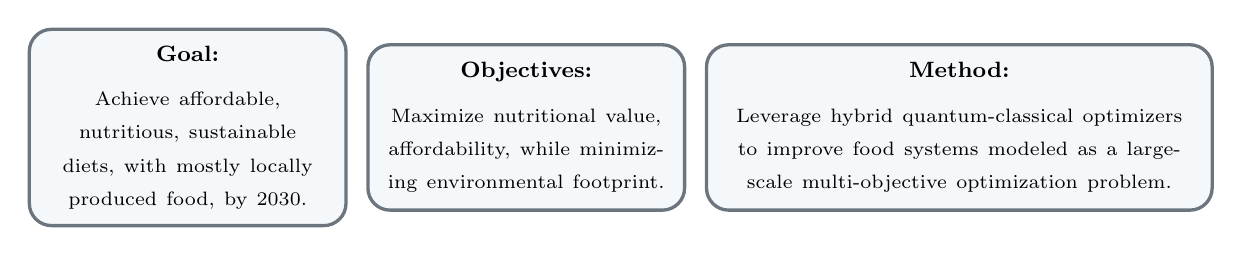
\begin{tikzpicture}
        % Goal box
        \node[rounded corners=8pt,fill=lightBg,draw=mutedGray,line width=1.2pt,
              text width=3.6cm,minimum height=2.1cm,align=center,inner sep=6pt] (goal) at (-0.1,0) {
            \footnotesize
            \textbf{Goal:}\\[4pt]
            \scriptsize
            Achieve affordable, nutritious, sustainable diets, with mostly locally produced food, by 2030.
        };
        
        % Objectives box
        \node[rounded corners=8pt,fill=lightBg,draw=mutedGray,line width=1.2pt,
              text width=3.6cm,minimum height=2.1cm,align=center,inner sep=6pt] (obj) at (4.2,0) {
            \footnotesize
            \textbf{Objectives:}\\[4pt]
            \scriptsize
            Maximize nutritional value, affordability, while minimizing environmental footprint.
        };
        
        % Method box
        \node[rounded corners=8pt,fill=lightBg,draw=mutedGray,line width=1.2pt,
              text width=6.0cm,minimum height=2.1cm,align=center,inner sep=6pt] (method) at (9.7,0) {
            \footnotesize
            \textbf{Method:}\\[4pt]
            \scriptsize
            Leverage hybrid quantum-classical optimizers to improve food systems modeled as a large-scale multi-objective optimization problem.
        };
    \end{tikzpicture}
    

\end{frame}


% ============================================================================
% SLIDE 3: CLASSICAL COMPUTATIONAL BOTTLENECKS
% ============================================================================
\begin{frame}{Classical Computational Bottlenecks}
    \framesubtitle{Why State-of-the-Art Solvers Struggle}
    
    \begin{columns}[T]
        \begin{column}{0.55\textwidth}
            \textbf{Classical MILP Solvers:}
            \begin{itemize}\footnotesize
                \item Branch-and-bound with LP relaxations
                \item Cutting-plane techniques (branch-and-cut)
                \item Primal heuristics for feasibility
            \end{itemize}
            
            \vspace{0.2cm}
            \textbf{Fundamental Bottlenecks:}
            \begin{enumerate}\scriptsize
                \item \textbf{LP relaxation weakness:} Large integrality gaps $\Rightarrow$ extensive tree exploration
                \item \textbf{Cutting-plane overhead:} Auxiliary LPs become expensive with diminishing returns
                \item \textbf{Tree explosion:} Exponential subproblem growth exhausts memory
                \item \textbf{Local minima traps:} Heuristics stuck in suboptimal regions
            \end{enumerate}
        \end{column}
        
        \begin{column}{0.43\textwidth}
            \vspace{0.3cm}
            \textbf{Crop Rotation Challenge:}
            \begin{itemize}\scriptsize
                \item \textbf{Quadratic objective} breaks LP structure
                \item \textbf{70--88\% frustrated pairs} create rugged landscape
                \item Poor bounds $\Rightarrow$ no effective pruning
            \end{itemize}
            
            \vspace{0.3cm}
            \begin{warnbox}
                \footnotesize\textbf{Result:} Gurobi times out on \textbf{85\%} of rotation scenarios (300s limit)
            \end{warnbox}
            
            \vspace{0.2cm}
            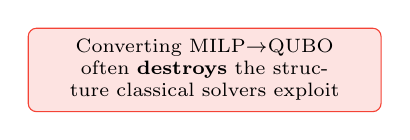
\begin{tikzpicture}
                \node[rounded corners=3pt,fill=alertRed!15,draw=alertRed,
                      font=\scriptsize,inner sep=4pt,text width=4.2cm,align=center] {
                    Converting MILP$\to$QUBO often \textbf{destroys} the structure classical solvers exploit
                };
            \end{tikzpicture}
        \end{column}
    \end{columns}
\end{frame}

% ============================================================================
% SLIDE 3B: QUANTUM COMPUTING OPPORTUNITY
% ============================================================================
\begin{frame}{The Quantum Computing Opportunity}
    \framesubtitle{Structure-Aware Hybrid Approaches}
    
    \begin{columns}[T]
        \begin{column}{0.55\textwidth}
            \textbf{Why Quantum for Hard Subproblems?}
            \begin{itemize}\footnotesize
                \item QUBO formulation native to quantum annealers
                \item \textbf{Quantum tunneling} escapes local minima
                \item Parallel exploration via superposition
                \item Favorable for sparse, frustrated interactions
            \end{itemize}
            
            \vspace{0.3cm}
            \textbf{Hybrid Strategy:}
            \begin{enumerate}\scriptsize
                \item Classical decomposition preserves structure
                \item Quantum component tackles \textbf{hard subproblems}
                \item Classical post-processing refines solutions
            \end{enumerate}
            
            \vspace{0.2cm}
            \begin{keyinsight}[Key Insight]
                \scriptsize Look for structural components that are \textbf{classically challenging} but naturally expressed as QUBO
            \end{keyinsight}
        \end{column}
        
        \begin{column}{0.43\textwidth}
            \vspace{0.2cm}
            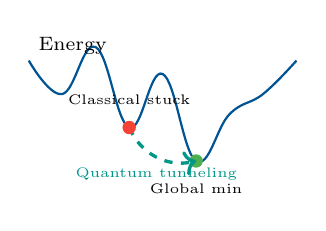
\begin{tikzpicture}[scale=0.85]
                % Energy landscape visualization
                \draw[thick,primaryBlue] plot[smooth,tension=0.7] coordinates {
                    (0,2) (0.5,1.5) (1,2.2) (1.5,1) (2,1.8) (2.5,0.5) (3,1.2) (3.5,1.5) (4,2)
                };
                \fill[accentGreen] (2.5,0.5) circle (0.1);
                \node[font=\tiny,below] at (2.5,0.3) {Global min};
                
                % Tunneling arrow
                \draw[->,accentTeal,very thick,dashed] (1.5,1) to[bend right=40] node[midway,below,font=\tiny] {Quantum tunneling} (2.5,0.5);
                
                % Classical stuck
                \fill[alertRed] (1.5,1) circle (0.1);
                \node[font=\tiny,above] at (1.5,1.2) {Classical stuck};
                
                \node[font=\scriptsize,anchor=north west] at (0,2.5) {Energy};
            \end{tikzpicture}
            
            \vspace{0.3cm}
            \begin{resultbox}
                \scriptsize\textbf{Crop rotation:} Frustrated constraints + quadratic synergies = ideal quantum candidate
            \end{resultbox}
            
            \vspace{0.2cm}
            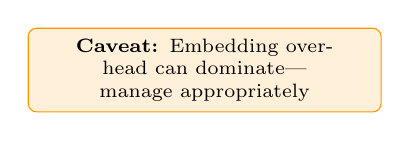
\begin{tikzpicture}
                \node[rounded corners=3pt,fill=warmOrange!15,draw=warmOrange,
                      font=\scriptsize,inner sep=4pt,text width=4.2cm,align=center] {
                    \textbf{Caveat:} Embedding overhead can dominate---manage appropriately
                };
            \end{tikzpicture}
        \end{column}
    \end{columns}
\end{frame}

% ============================================================================
% SLIDE 4: OQI PIPELINE & APPROACH
% ============================================================================
\begin{frame}{Three Complementary Studies}
    
    \centering
    
\begin{tikzpicture}[
        study/.style={rounded corners=8pt,minimum width=4.2cm,minimum height=2.5cm,
                     font=\scriptsize,align=center,text=white,
                     drop shadow={opacity=0.3,shadow xshift=1mm,shadow yshift=-1mm}},
        legend/.style={rounded corners=6pt,fill=white,draw=mutedGray,align=center,font=\scriptsize,inner sep=6pt}
    ]
        % Study 1
        \node[study,fill=primaryBlue] (s1) at (0,1.2) {
            \Large\faServer\\[4pt]
            \normalsize\textbf{Study 1.A}\\[2pt]
            \small Hybrid Solver\\
            Benchmarking\\[4pt]
            \scriptsize Variant 1.A\\
        };
        
        % Study 2
        \node[study,fill=accentTeal] (s2) at (5,1.2) {
            \Large\faMicrochip\\[4pt]
            \normalsize\textbf{Study 2.A}\\[2pt]
            \small Pure QPU\\
            Decomposition\\[4pt]
            \scriptsize Variant 2.A\\
        };
        
        % Study 3
        \node[study,fill=accentGreen] (s3) at (10,1.2) {
            \Large\faRocket\\[4pt]
            \normalsize\textbf{Study 2.B}\\[2pt]
            \small Quantum\\
            Improvement\\[4pt]
            \scriptsize Variant 2.B\\
        };
        
        % Arrows
        \draw[->,very thick,primaryBlue!60] (s1.east) -- (s2.west);
        \draw[->,very thick,accentTeal!60] (s2.east) -- (s3.west);
    \end{tikzpicture}
    
    \vspace{0.5cm}  % Increased from 0.5cm
    
    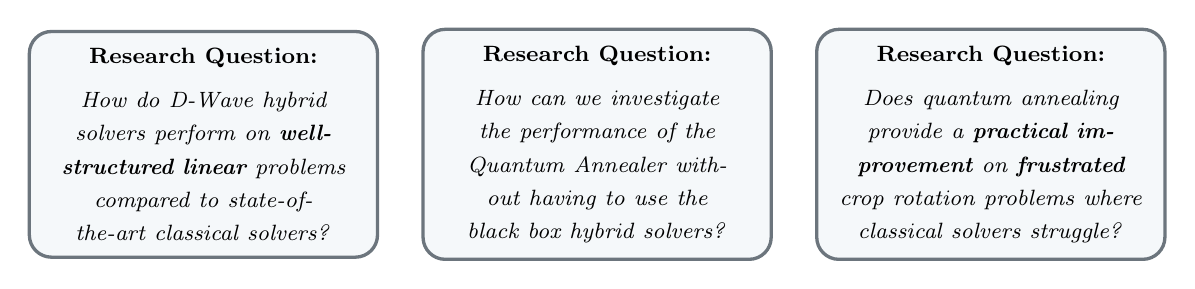
\begin{tikzpicture}[
        study/.style={rounded corners=8pt,minimum width=4.2cm,minimum height=2.5cm,
                     font=\scriptsize,align=center,text=white,
                     drop shadow={opacity=0.3,shadow xshift=1mm,shadow yshift=-1mm}},
        legend/.style={rounded corners=6pt,fill=white,draw=mutedGray,align=center,font=\scriptsize,inner sep=6pt}
    ]
        % Study 1
        \node[rounded corners=8pt,fill=lightBg,draw=mutedGray,line width=1.2pt,
              text width=4.0cm,minimum height=2.1cm,align=center,inner sep=6pt] (s1) at (0,-2.30) {
            \centering\footnotesize
            \textbf{Research Question:}\\[4pt]
            \textit{How do D-Wave hybrid solvers perform on \textbf{well-structured linear} problems compared to state-of-the-art classical solvers?}
        };
        
        % Study 2
        \node[rounded corners=8pt,fill=lightBg,draw=mutedGray,line width=1.2pt,
              text width=4.0cm,minimum height=2.1cm,align=center,inner sep=6pt] (s2) at (5,-2.30) {
            \centering\footnotesize
            \textbf{Research Question:}\\[4pt]
                \textit{How can we investigate the performance of the Quantum Annealer without having to use the black box hybrid solvers?}
        };
        
        % Study 3
        \node[rounded corners=8pt,fill=lightBg,draw=mutedGray,line width=1.2pt,
              text width=4.0cm,minimum height=2.1cm,align=center,inner sep=6pt] (s3) at (10,-2.30) {
            \centering\footnotesize
            \textbf{Research Question:}\\[4pt]
                \textit{Does quantum annealing provide a \textbf{practical improvement} on \textbf{frustrated} crop rotation problems where classical solvers struggle?}
        };
        
    \end{tikzpicture}
    
\end{frame}

% ============================================================================
% SLIDE 5: KEY RESULTS - THREE STUDIES COMPARISON
% ============================================================================
\begin{frame}{Key Results: Classical vs Quantum Performance}
    \framesubtitle{Three Studies, Three Different Conclusions}
    
\vspace{-0.3cm}
\begin{columns}[T]

% Study 1.A Column
\begin{column}{0.32\textwidth}
\begin{block}{\centering\small\faServer\ Study 1.A: Hybrid Solvers}
\vspace{0.1cm}
\textbf{\scriptsize Problem:} Variant A (Linear)\\
\textbf{\scriptsize Scale:} 10--1,000 farms

\vspace{0.15cm}
\textbf{\scriptsize Gurobi:}
\begin{itemize}\tiny
    \item[\textcolor{accentGreen}{\faCheck}] Optimal in \textbf{$<$1.2s}
    \item[\textcolor{accentGreen}{\faCheck}] 0\% MIP gap
\end{itemize}

\textbf{\scriptsize D-Wave Hybrid:}
\begin{itemize}\tiny
    \item[\textcolor{warmOrange}{\faTimes}] 5.3--5.5s constant
    \item[\textcolor{warmOrange}{\faTimes}] QPU only 1.3\% of time
\end{itemize}

\vspace{0.1cm}
\centering
\textcolor{accentGreen}{\large\faTrophy}\\
\tiny\textbf{Winner: Gurobi}
\end{block}
\end{column}

% Study 2.A Column
\begin{column}{0.32\textwidth}
\begin{block}{\centering\small\faMicrochip\ Study 2.A: Pure QPU}
\vspace{0.1cm}
\textbf{\scriptsize Problem:} Variant A (Linear)\\
\textbf{\scriptsize Scale:} 10--1,000 farms

\vspace{0.15cm}
\textbf{\scriptsize QPU Performance:}
\begin{itemize}\tiny
    \item[\textcolor{accentGreen}{\faCheck}] Linear $O(f)$ scaling
    \item[\textcolor{accentGreen}{\faCheck}] $<$2\% chain breaks
\end{itemize}

\textbf{\scriptsize Bottleneck:}
\begin{itemize}\tiny
    \item[\textcolor{alertRed}{\faTimes}] 95--99\% embedding overhead
    \item[\textcolor{warmOrange}{\faTimes}] 31--57\% solution gap
\end{itemize}

\vspace{0.1cm}
\centering
\textcolor{accentGreen}{\large\faTrophy}\\
\tiny\textbf{Winner: Gurobi}
\end{block}
\end{column}

% Study 2.B Column
\begin{column}{0.32\textwidth}
\begin{block}{\centering\small\faRocket\ Study 2.B: Rotation}
\vspace{0.1cm}
\textbf{\scriptsize Problem:} Variant B (Quadratic)\\
\textbf{\scriptsize Scale:} 5--200 farms

\vspace{0.15cm}
\textbf{\scriptsize Gurobi:}
\begin{itemize}\tiny
    \item[\textcolor{alertRed}{\faTimes}] 85\% timeout (300s)
    \item[\textcolor{alertRed}{\faTimes}] 16,308\% avg MIP gap
\end{itemize}

\textbf{\scriptsize QPU Hierarchical:}
\begin{itemize}\tiny
    \item[\textcolor{accentGreen}{\faCheck}] Completes all instances
    \item[\textcolor{accentGreen}{\faCheck}] \textbf{3.80$\times$} better benefit
\end{itemize}

\vspace{0.1cm}
\centering
\textcolor{primaryBlue}{\large\faTrophy}\\
\tiny\textbf{Winner: QPU}
\end{block}
\end{column}

\end{columns}

\vspace{0.3cm}
\begin{keybox}
\centering
\small\textbf{Key Insight:} Neither approach universally dominates. Optimal solver depends on \textbf{problem structure} (linear vs quadratic, frustrated constraints), not just size.
\end{keybox}
\end{frame}

% ============================================================================
% SLIDE 6: CONCLUSION & INDUSTRY RELEVANCE
% ============================================================================
\begin{frame}{Conclusion \& Industry Relevance}
    \framesubtitle{When Quantum Computing Makes a Difference}
    
    \begin{columns}[T]
        \begin{column}{0.48\textwidth}
            \textbf{Key Findings:}
            \begin{enumerate}\footnotesize
                \item \textcolor{primaryBlue}{\textbf{Formulation matters}}: Quantum excels on frustrated QUBO problems
                \item \textcolor{accentTeal}{\textbf{Linear scaling}}: Pure QPU time scales $O(n)$
                \item \textcolor{accentGreen}{\textbf{3.80$\times$ improvement}}: On rotation problems where classical fails
                \item \textcolor{warmOrange}{\textbf{Diverse solutions}}: Quantum naturally produces agriculturally robust allocations
            \end{enumerate}
            
            \vspace{0.3cm}
            
        \end{column}
        
        \begin{column}{0.50\textwidth}
            \textbf{Industry Applications:}
            
            \begin{tikzpicture}[
                app/.style={rounded corners=2pt,fill=accentGreen!15,draw=accentGreen,
                           font=\scriptsize,inner sep=4pt,minimum width=5.3cm,align=left}
            ]
                \node[app] at (0,0) {\faIndustry\ \textbf{AgriTech:} Large-scale crop planning};
                \node[app] at (0,-0.65) {\faTruck\ \textbf{Supply Chain:} Multi-period logistics};
                \node[app] at (0,-1.3) {\faChartLine\ \textbf{Finance:} Portfolio with constraints};
                \node[app] at (0,-1.95) {\faCity\ \textbf{Urban Planning:} Resource allocation};
            \end{tikzpicture}
            
        \end{column}
    \end{columns}
\begin{keyinsight}[Take-Home Message]
\centering
                \scriptsize Quantum annealing is a valid choice for multi-objective agricultural optimization with frustrated constraints.
            \end{keyinsight}
\end{frame}

% ============================================================================
% CLOSING SLIDE
% ============================================================================
{
\setbeamertemplate{headline}{}
\setbeamertemplate{footline}{}
\begin{frame}[plain]
\begin{tikzpicture}[remember picture,overlay]
    % Background
    \node[inner sep=0,anchor=center] at (current page.center)
    {\includegraphics[width=\paperwidth,height=\paperheight]{images/OQI background.jpeg}};

  % Optional: semi-transparent overlay to improve text contrast
  \fill[black,opacity=0.35] (current page.south west) rectangle (current page.north east);
    
    % Main content
    \node[white,font=\fontsize{40}{44}\selectfont\bfseries] at ([yshift=1.5cm]current page.center) {Thank You};
    
    \node[white!90,font=\Large] at ([yshift=0.3cm]current page.center) {Questions \& Discussion};
    
    % Contact info
    \node[rounded corners=5pt,fill=white!10,text=primaryBlue,font=\normalsize,inner sep=10pt] 
        at ([yshift=-1.5cm]current page.center) {
        $\bullet$\quad edoardo.spigarolo@epfl.ch 
    };
    
    % Institution
    \node[white!60,font=\small] at ([yshift=-2.8cm]current page.center) 
        {$\bullet$\quad Open Quantum Institute};
    
    % Bottom icons
    \node[white!50,font=\small] at ([yshift=0.5cm]current page.south) 
        {\faGithub\quad \faEnvelope\quad \faGlobe};
\end{tikzpicture}
\end{frame}
}

\end{document}